\subsection{Distribuzione gaussiana}

\subsubsection{Variabile aleatoria gaussiana}

\begin{Mybox}
    \begin{definizione}
     Una variabile aleatoria continua $X$ dicesi \emph{gaussiana}, o \emph{normale}, se è descritta dalla seguente \emph{pdf}:
    \begin{equation}
        p(x)=\frac{1}{\sqrt{2 \pi \sigma^2}} \exp \Biggl(-\frac{(x-\mu)^2}{2 \sigma^2}\Biggr)
    \end{equation}    
    \end{definizione}
\end{Mybox}


\noindent Sinteticamente si scrive 
\[
    X \sim \mathcal{N}(\mu, \sigma^2) 
\]
per evidenziare come la \emph{pdf} di una \emph{v.a}.\ gaussiana sia completamente determinata qualora vengano assegnati i due parametri seguenti: 
\begin{itemize}
    \item $\mu=\mathbb{E}[X]\in \mathbb{R}$, la \emph{media statistica} della \emph{v.a}.\ $X$.
    \item $\sigma^2=\mathbb{V}ar[X]$, la \emph{varianza} della \emph{v.a}.\ $X$.
\end{itemize} 

\begin{figure}
    \centering
    \subfloat[][\emph{pdf} di una variabile aleatoria gaussiana standard, $X \sim \mathcal{N}(0, 1)$.]
   {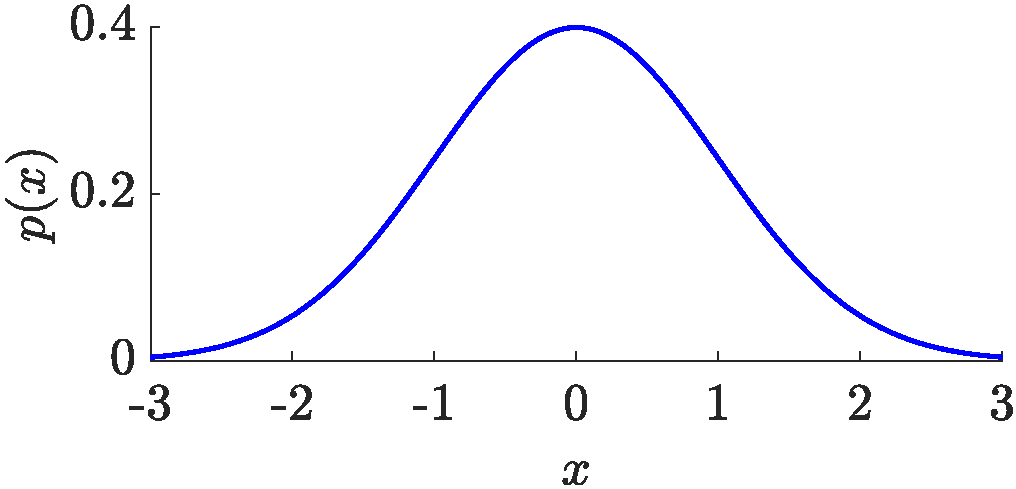
\includegraphics[keepaspectratio, scale=0.38]{normal1D1}} \quad
    \subfloat[][\emph{pdf} di variabili gaussiane con $\mu=2$ e $\sigma^2=4,1,0.25$]
   {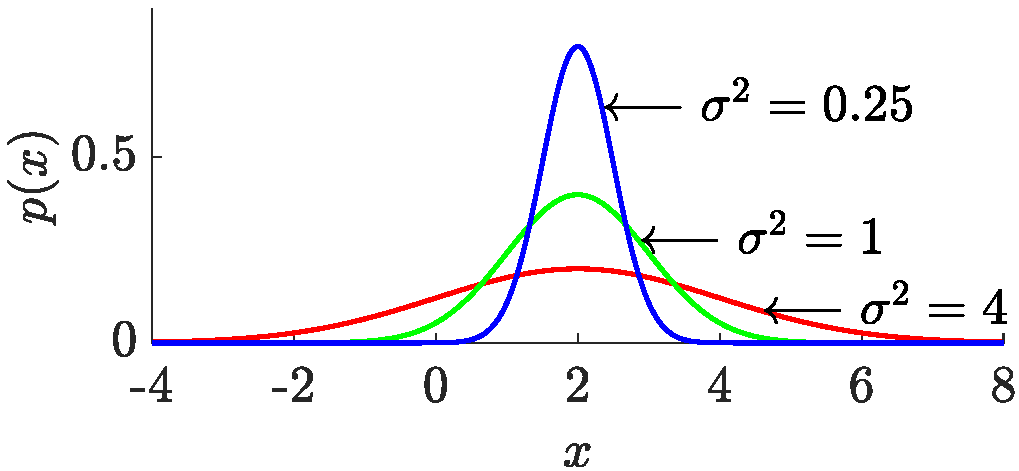
\includegraphics[keepaspectratio, scale=0.38]{normal1D2}} 
  \caption{Distribuzioni gaussiane unidimensionali}
\label{fig:normali1D}
\end{figure}

\smallskip 

\noindent Si noti (Figura~\ref{fig:normali1D}) la peculiare forma, tipica di una “campana”, esibita dalla \emph{pdf} di una gaussiana (\emph{bell-shaped pdf}). 
Dalla Figura~\ref{fig:normali1D} è possibile desumere il significato dei due suddetti parametri:
\begin{itemize}
    \item $\mu$ è un \emph{fattore di posizione} che costituisce il centro di simmetria della densità di probabilità.
    Modifiche apportate a tale parametro si riflettono in traslazioni orizzontali rigide della \emph{pdf}. 
    \item $\sigma^2$ è un \emph{fattore di scala} che regola la larghezza della campana attorno alla media $\mu$: all'aumentare di $\sigma^2$ 
    la campana si allarga e diventa più schiacciata (per preservare l'unitarietà dell'area sottesa), mentre 
    al diminuire di $\sigma^2$ corrisponde una campana più stretta e alta (Figura~\ref{fig:normali1D}).
\end{itemize} 



%---------------------------------------------------------------------------------

\subsubsection{Vettore aleatorio gaussiano}

\begin{figure}
    \centering
    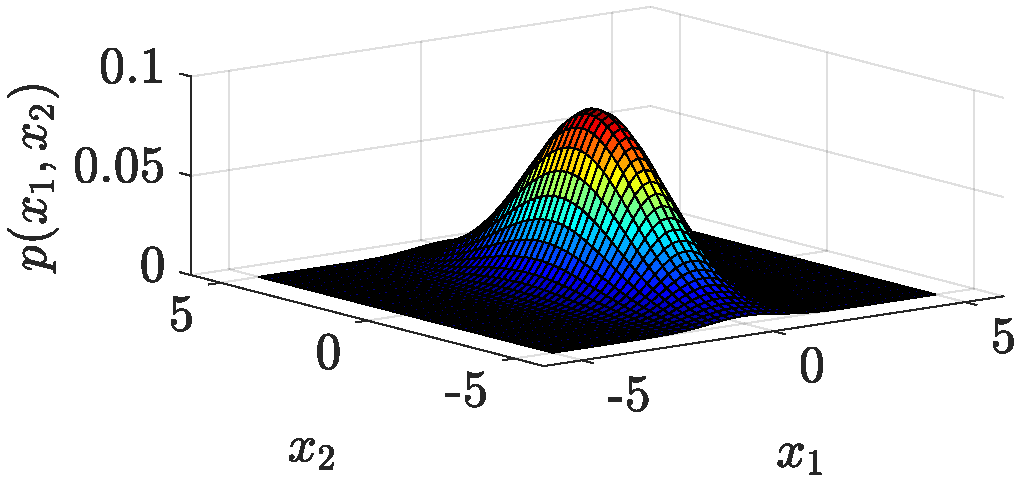
\includegraphics[keepaspectratio, scale=0.55]{multivariate_normal}
    \caption{Distribuzione gaussiana bidimensionale}
\end{figure}


\begin{Mybox}
    \begin{definizione}
        Un vettore aleatorio $\mathbf{X}=[X_1,\dots,X_N]^T \in \mathbb{R}^N$ dicesi \emph{gaussiano}, o \emph{normale}, qualora abbia la seguente \emph{pdf}:
        \begin{equation}
               p(\mathbf{x})=\frac{1}{(2\pi)^{N/2}\lvert  \mathbf{\Sigma} \rvert^{1/2} }\exp \biggl(-\frac{1}{2}(\mathbf{x}-\bm{\mu})^{T} \mathbf{\Sigma}^{-1}(\mathbf{x}-\bm{\mu})\biggr)
        \end{equation}
        dove $\mathbf{x}=[x_1,\dots,x_N]^T \in \mathbb{R}^N$ e $\lvert \mathbf{\Sigma} \rvert = \text{det}(\mathbf{\Sigma})$ è il determinante della matrice $\mathbf{\Sigma}$.    
    \end{definizione}
\end{Mybox}

\noindent Sinteticamente si scrive 
\[
    \mathbf{X} \sim \mathcal{N}(\bm{\mu}, \mathbf{\Sigma}) \quad\text{o}\quad p(\mathbf{x})=\mathcal{N}(\mathbf{x};\bm{\mu}, \mathbf{\Sigma})
\]
per evidenziare come la \emph{pdf} del vettore aleatorio $X$ sia completamente determinata qualora vengano assegnati: 
\begin{itemize}
    \item il \emph{vettore delle medie} $\bm{\mu}=\mathbb{E}[\mathbf{X}]=(\mathbb{E}[X_1],\mathbb{E}[X_2],\dots,\mathbb{E}[X_N])^T$.
    \item la \emph{matrice di covarianza} $\mathbf{\Sigma}= \mathbb{E}[(\mathbf{X}-\bm{\mu})(\mathbf{X}-\bm{\mu})^T]\in \mathbb{R}^{N \times N}$.
\end{itemize} 
\smallskip
\begin{oss}[Combinazione lineare di vettori gaussiani indipendenti]\label{oss:comb_lin_normali}
    Siano $\mathbf{X}\sim\mathcal{N}(\bm{\mu}_{\mathbf{X}}, \bm{\Sigma}_{\mathbf{X}})$ e 
    $\mathbf{Y}\sim\mathcal{N}(\bm{\mu}_{\mathbf{Y}}, \bm{\Sigma}_{\mathbf{Y}})$ due vettori aleatori gaussiani \emph{indipendenti}. Siano, inoltre,
    $\bm{A}$ e $\bm{B}$ due matrici. Sussiste il seguente risultato:
    \begin{equation}
     (\bm{A}\mathbf{X}+\bm{B}\mathbf{Y}) \sim \mathcal{N}(\bm{A}\bm{\mu}_{\mathbf{X}} +\bm{B}\bm{\mu}_{\mathbf{Y}}, \bm{A}\bm{\Sigma}_{\mathbf{X}}\bm{A}^T+\bm{B}\bm{\Sigma}_{\mathbf{Y}}\bm{B}^T) \label{eq:comblingauss}
    \end{equation}
    da cui si evince che la combinazione lineare di vettori aleatori gaussiani indipendenti è ancora un vettore aleatorio gaussiano.
    La~\eqref{eq:comblingauss} declinata al caso in cui le suddette matrici siano degli scalari diventa:
    \begin{equation}
        (a\mathbf{X}+b\mathbf{Y}) \sim \mathcal{N}(a\bm{\mu}_{\mathbf{X}} +b\bm{\mu}_{\mathbf{Y}}, a^2\bm{\Sigma}_{\mathbf{X}}+b^2\bm{\Sigma}_{\mathbf{Y}})\label{eq:comblingauss_scalar}
    \end{equation}
\end{oss}

\subsubsection{Trasformazione affine di una v.a.\ gaussiana}
\label{sssec:Reparametrization_Trick}


\begin{Mybox}
    Una variabile aleatoria gaussiana $X \sim \mathcal{N}(\mu, \sigma^2)$ può essere sempre riguardata come
    una \emph{trasformazione affine} (cascata di cambiamento di scala e traslazione) di una 
    \emph{gaussiana standard} $X_0 \sim \mathcal{N}(0, 1)$
    \begin{equation}
        X = \sigma X_0 + \mu,  \qquad \sigma>0, \, \mu \in \mathbb{R} \label{eq:rep_trick}
    \end{equation}
\end{Mybox}
